%% LyX 2.4.4 created this file.  For more info, see https://www.lyx.org/.
%% Do not edit unless you really know what you are doing.
\documentclass[english,t]{beamer}
\usepackage{mathptmx}
\usepackage[T1]{fontenc}
\usepackage[latin9]{inputenc}
\usepackage{amstext}
\usepackage{amssymb}
\usepackage{cancel}
\PassOptionsToPackage{normalem}{ulem}
\usepackage{ulem}

\makeatletter

%%%%%%%%%%%%%%%%%%%%%%%%%%%%%% LyX specific LaTeX commands.
%% Because html converters don't know tabularnewline
\providecommand{\tabularnewline}{\\}

%%%%%%%%%%%%%%%%%%%%%%%%%%%%%% Textclass specific LaTeX commands.
% this default might be overridden by plain title style
\newcommand\makebeamertitle{\frame{\maketitle}}%
% (ERT) argument for the TOC
\AtBeginDocument{%
  \let\origtableofcontents=\tableofcontents
  \def\tableofcontents{\@ifnextchar[{\origtableofcontents}{\gobbletableofcontents}}
  \def\gobbletableofcontents#1{\origtableofcontents}
}

%%%%%%%%%%%%%%%%%%%%%%%%%%%%%% User specified LaTeX commands.
\usetheme{Warsaw}
% or ...

\setbeamercovered{transparent}
% or whatever (possibly just delete it)
\setbeamercovered{invisible} %makes overlays invisible

%gets rid of navigation symbols
\setbeamertemplate{navigation symbols}{}

%\usepackage{hyperref}
%\usepackage[usenames,dvipsnames,table]{xcolor} %adds additional color options
\definecolor{links}{HTML}{2A1B81}
%\hypersetup{colorlinks,linkcolor=blue,urlcolor=links}

\usepackage{multicol}

\usepackage{tikz}
\usetikzlibrary{calc}
\usetikzlibrary{plotmarks}
\usetikzlibrary{shapes}
\usepackage{pgfplots}
\pgfplotsset{compat=newest}

\usepackage{forest} %%for tree diagram

\usepackage{calc}
\usepackage[nomessages]{fp}

%\usepackage{advdate}    % Advancing/saving dates
\usepackage{datetime}   % Dates formatting
%\usepackage{datenumber} % Counters for dates

\usepackage[super]{nth}

\usepackage{etex}

\usepackage{fancybox}

\usepackage[outline]{contour}  %allows text halos
\contourlength{1pt} %sets halo width
%%example: \node at (0.75,0.5) {\contour{white}{\Large Text!}};
%%example:  \node [fill=white,inner sep=1pt] at (2.25,0.5) {\Large 			Text!};
%%example:  \node [fill=white,rounded corners=2pt,inner sep=1pt] at 			(3.75,0.5) {\Large Text!};

%%%%%%%%%%%%%%%%%%%%%%%%%%%
\def\formatdateny{\csname noyear\languagename\expandafter\endcsname\formatdate}
\def\noyearenglish#1, \the\@year{#1}
\let\noyearamerican\noyearenglish
\let\noyearbritish\noyearenglish

%%allows uncover with forest diagrams
\tikzset{
    invisible/.style={opacity=0,text opacity=0},
    visible on/.style={alt=#1{}{invisible}},
    alt/.code args={<#1>#2#3}{%
      \alt<#1>{\pgfkeysalso{#2}}{\pgfkeysalso{#3}} % \pgfkeysalso doesn't change the path
    },
}
\forestset{
  visible on/.style={
    for tree={
      /tikz/visible on={#1},
      edge={/tikz/visible on={#1}}}}}

%%%redefines column alignment to match vertically
%\define@key{beamerframe}{t}[true]{% top
  %\beamer@frametopskip=.2cm plus .5\paperheight\relax%
  %\beamer@framebottomskip=0pt plus 1fill\relax%
 % \beamer@frametopskipautobreak=\beamer@frametopskip\relax%
  %\beamer@framebottomskipautobreak=\beamer@framebottomskip\relax%
  %\def\beamer@initfirstlineunskip{}%
%}

%%provides pdf with 4 slides per page; don't forget to add 'handout' to remove overlays
%\usepackage{pgfpages}
%\pgfpagesuselayout{4 on 1}[a4paper, landscape, border shrink=7mm]
%\pgfpageslogicalpageoptions{1}{border code=\pgfusepath{stroke}}
%\pgfpageslogicalpageoptions{2}{border code=\pgfusepath{stroke}}
%\pgfpageslogicalpageoptions{3}{border code=\pgfusepath{stroke}}
%\pgfpageslogicalpageoptions{4}{border code=\pgfusepath{stroke}}
%%%Don't forget to add 'handout'

\makeatother

\usepackage{babel}
\begin{document}
\newcommand{\xmax}{2000}
\newcommand{\xmin}{0}
\newcommand{\xstep}{0} %must be xmin+n
\newcommand{\ymax}{500}
\newcommand{\ymin}{0}
\newcommand{\ystep}{0} %must be ymin+n

\newcounter{countEx} \setcounter{countEx}{0}
\newcounter{countProb} \setcounter{countProb}{0}
\resetcounteronoverlays{countEx} \resetcounteronoverlays{countProb}

\newcommand{\ex}[3]{
	\addtocounter{countEx}{1}
	\only<#1-#2>{\begin{exampleblock} {Example \chNum.\secNum.\arabic{countEx}.} #3	\end{exampleblock}}
}

\newcommand{\prob}[4]{
	\addtocounter{countProb}{1}
	\only<#1-#2>{\begin{exampleblock} {Problem  \chNum.\secNum.\arabic{countProb}.\,#3} #4	\end{exampleblock}}
}

\newcommand{\yline}[4]{
	(#2 - #4)/(#1 - #3)*(x - #1) + #2
}

\beamerdefaultoverlayspecification{<+->}

%%%%Chapter and Section numbers%%%%%
\newcommand{\chNum}{1}
\newcommand{\secNum}{2}
\newcommand{\secTitle}{Symbolic Logic}

\title[Section \chNum.\secNum: \secTitle]{Section \chNum.\secNum: \secTitle}

\subtitle{Finite Mathematics~~MTH 107~~Fall 2014}

\author{Dr.\,James Ashe}

\titlegraphic{\includegraphics[height=2.75cm]{/home/jim/JamesAshe/MHU/images/MarsHilUniversityLogo-Virtical.png}}

\date{\formatdate{12}{9}{2014} and \formatdate{15}{9}{2014}}

\institute{Mars Hill University}

\makebeamertitle 
\begin{frame}{Symbolic Logic}

\begin{block}{Statement}
A \emph{statement }is a declarative sentence that is either true
or false. 
\end{block}
\begin{columns}


\column{5.5cm}
\begin{itemize}
\item <2->Socrates was a man. \uncover<6->{\textbf{T}}
\item <3->$8-3+4=1$ \uncover<7->{\textbf{F}}
\item <4->A triangle has three sides. \uncover<8->{\textbf{T}}
\item <5->[]\uline{STATEMENTS: True or False}
\end{itemize}

\column{5.5cm}
\begin{itemize}
\item <9->Is Socrates a man?
\item <10->Socrates was a bad man.
\item <11->Go do some math.
\item <12->$8-3+4$
\item <13->This statement is false (\emph{Liar's Paradox}). 
\item <14->$A$ and not $A$.
\item <15->[]\uline{NOT STATEMENTS}
\end{itemize}
\end{columns}
\end{frame}

\begin{frame}{Compound Statements}

\begin{block}{Compound Statement}
A \emph{compound statement} is two or more statements combined.

\begin{itemize}
\item <2->Combined with \emph{logical connectives}, e.g.,\emph{ }and, or,
not, yet, if, then,...
\item <3->The simple statements that compose a compound statement are called
\emph{component} statements.
\end{itemize}
\end{block}
\vspace{-.5cm}
\begin{columns}


\column{6cm}
\begin{itemize}
\item <4->Socrates was a man, and Theano was a woman. 
\item <5->If a polygon has three sides then it is a triangle.
\item <6->$8-3+4=9$ not $1$.
\item <7->[]\uline{COMPOUND STATEMENTS}
\end{itemize}

\column{6cm}
\begin{itemize}
\item <8->Is Socrates a man or woman?
\item <9->If a polygon has three sides then go get some ice cream.
\item <10->Truth or dare is a game.
\item <11->This statement is true, and this statement is false. 
\item <12->[]\uline{NOT COMPOUND STATEMENTS}
\end{itemize}
\end{columns}
\end{frame}

\begin{frame}{Your Turn: Statements}

\prob{1}{1}{Decide whether the following is a statement. If it is a statement, decide whether or not it is compound}{Nashville is the capital of Tennessee.}

\prob{2}{2}{Decide whether the following is a statement. If it is a statement, decide whether or not it is compound}{Got milk?}

\prob{3}{3}{Decide whether the following is a statement. If it is a statement, decide whether or not it is compound}{China does not have a population of more than 1 billion, and it is a country.}

\prob{4}{4}{Decide whether the following is a statement. If it is a statement, decide whether or not it is compound}{If I get an \emph{A}  then I will celebrate.}
\end{frame}

\begin{frame}{Negation}

\begin{block}<2->{Negation}
The \emph{negation }of a true statement makes it false, and the
\emph{negation }of a false statement is true.
\end{block}
\vspace{-.5cm}
\begin{columns}


\column{5cm}
\begin{itemize}
\item <2->[]\textbf{Statement}

\begin{itemize}
\item <2->Socrates is a man. 
\item <4->Socrates is not a man.
\item <6->$8-3+4=9$
\item <8->$3<4$, ``$3$ is less than $4$''
\item <10->All men are mortal.
\item <12->No men are mortal.
\end{itemize}
\end{itemize}

\column{7.5cm}
\begin{itemize}
\item <3->[]\textbf{Negation of Statement}

\begin{itemize}
\item <3->Socrates is not a man.
\item <5->Socrates is a man.
\item <7->$8-3+4\neq9$
\item <9->$3\geq4$, ``$3$ is greater than or equal to $4$''
\item <11->Some men are not mortal.
\item <13->Some men are mortal.
\end{itemize}
\end{itemize}
\end{columns}
\end{frame}

\begin{frame}{Your Turn: Negation}

\prob{1}{}{Write a negation of each statement.}{This is not the time to complain.}\prob{2}{}{Write a negation of each statement.}{$y\leq 5$}\prob{3}{}{Write a negation of each statement}{Some of the beverages contain caffeine.}\prob{4}{}{Write a negation of each statement}{None of the beverages contain caffeine.}\prob{4}{}{Write a negation of each statement}{All of the beverages contain caffeine.}\prob{5}{}{Write a negation of each statement}{Some of the beverages do not contain caffeine.}
\end{frame}

\begin{frame}{Symbolic Logic}

\begin{columns}


\column{4.25cm}
\begin{block}{Notation}

\begin{tabular}{rl}
 & \textbf{Symbol}\tabularnewline
statement & $p$, $q$, $r$, etc.\tabularnewline
``and'' & $\wedge$\tabularnewline
``or'' & $\vee$\tabularnewline
``not'' & $\sim$\tabularnewline
\end{tabular}
\end{block}

\column{6.5cm}

\uncover<2->{Let $m$ represent ``Socrates is a man'' and $r$
represent ``it's going to rain''.}
\begin{itemize}
\item <2->[ex.]\emph{Socrates is a man and it's going to rain.}

\begin{itemize}
\item []<3->$m\wedge r$
\end{itemize}
\item <4->[ex.]\emph{Socrates is }not \emph{a man or it's going to rain.}

\begin{itemize}
\item []<5->$\sim m\vee r$
\end{itemize}
\item <6->[ex.]\emph{It is not case that Socrates is a man or it's going
to rain.}

\begin{itemize}
\item []<7->$\sim(m\vee r)$
\item []<8->Equivalently, $\sim m\wedge\sim r$, \emph{Socrates is not
a man and it is not going to rain}.
\end{itemize}
\end{itemize}
\end{columns}
\end{frame}

\begin{frame}{Conditional Statements}

\vspace{-.5cm}
\begin{columns}


\column{4.75cm}
\begin{block}{Notation}

\begin{tabular}{rl}
 & \textbf{Symbol}\tabularnewline
statement & $p$, $q$, $r$, etc.\tabularnewline
``$p$ and $q$'' & $p\wedge q$\tabularnewline
``$p$ or $q$'' & $p\vee q$\tabularnewline
``not $p$'' & $\sim p$\tabularnewline
``if $p$ then $q$'' & $p\rightarrow q$\tabularnewline
\end{tabular}
\end{block}

\column{6.5cm}

\uncover<2->{$p$: It is a mammal\\
$q$: It is warm blooded.}
\begin{itemize}
\item <2->[ex.]\emph{If it is a mammal then it is warm blooded.}

\begin{itemize}
\item []<3->$p\rightarrow q$
\end{itemize}
\item <4->[ex.]\emph{If it is not warmblooded then it is not a mammal.}

\begin{itemize}
\item []<5->$\sim q\rightarrow\sim p$ (contrapositive)
\end{itemize}
\item <6->[ex.]\emph{All mammals are warm blooded.}
\item <8->[ex.]\emph{No snakes are warm blooded.}

\begin{itemize}
\item []<9->$s\rightarrow\sim q$
\end{itemize}
\end{itemize}
\end{columns}
\begin{exampleblock}<3-9>{} \begin{center}

\only<3-3>{''\Ovalbox{If} $\underset{p\equiv\mbox{premise}}{\underbrace{\mbox{it is a mammal}}}$
\Ovalbox{then} $\underset{q\equiv\mbox{conclusion}}{\underbrace{\mbox{it is warm blooded}}."}$}

\only<7-7>{''\Ovalbox{If} $\underset{p\equiv\mbox{premise}}{\underbrace{\mbox{it is a mammal}}}$
\Ovalbox{then} $\underset{q\equiv\mbox{conclusion}}{\underbrace{\mbox{it is warm blooded}}."}$}

\only<9-9>{''\Ovalbox{If} $\underset{s\equiv\mbox{premise}}{\underbrace{\mbox{it is a snake}}}$
\Ovalbox{then} $\underset{\sim q\equiv\mbox{conclusion}}{\underbrace{\mbox{it is \textbf{not }warm blooded}}."}$}

\end{center}
\end{exampleblock}
\end{frame}

\begin{frame}{Necessary and Sufficient}

\vspace{-.5cm}
\begin{block}{}\begin{center}% 
	\begin{tabular}{ccc} 
		\only<1-4>{\Ovalbox{Sufficient Condition}} \only<5->{\Ovalbox{Necessary Condition}} & 
		\only<1-4>{$\longrightarrow$} \only<5->{$\longleftarrow$} & 
		\only<1-4>{\Ovalbox{Necessary Condition}} \only<5->{\Ovalbox{Sufficient Condition}}
	\tabularnewline 
		\only<1-4>{\textcolor{red}{$p$: hypothesis}} \only<5->{\textcolor{red}{$q$: conclusion}} & 
		\only<1-4>{\textcolor{red}{$p$ implies $q$}} \only<5->{\textcolor{red}{$q$ implies $p$}} & 
		\only<1-4>{\textcolor{red}{$q$: conclusion}} \only<5->{\textcolor{red}{$p$: hypothesis}}
	\tabularnewline 
	\end{tabular}
\end{center}
\end{block}

\begin{columns}


\column{4.75cm}

%%%%little circle in big%%%%%
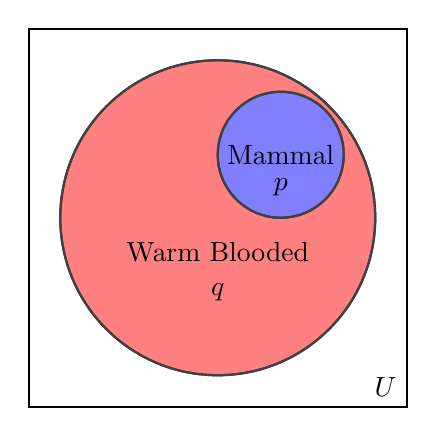
\begin{tikzpicture}[scale=.8]
	\def\circleA{(1,-1) circle (2.5)} %A
	\def\circleB{(0:2) circle (1)} %B

	\colorlet{circle edgeA}{black!75} 
	\colorlet{circle areaA}{red!50}
	\colorlet{circle edgeB}{black!75} 
	\colorlet{circle areaB}{blue!50}

	\tikzset{
		filledA/.style={fill=circle areaA, draw=circle edgeA, thick},
		filledB/.style={fill=circle areaB, draw=circle edgeB, thick},
		outlineA/.style={draw=circle edgeA, thick},
		outlineB/.style={draw=circle edgeB, thick},
	}

	\begin{scope}[fill opacity=1.0]         
			\fill[filledA] \circleA;
			\fill[filledB] \circleB;    
	\end{scope}

	\draw[outlineA] \circleA node[below = 5pt] {Warm Blooded} node[below = 20pt] {$q$}; 
	\draw[outlineB] \circleB node {Mammal} node[below = 5pt] {$p$};
	%\node[anchor=south] at (current bounding box.north) {$A \cup B$}; 
	\draw[thick] (-2,-4) rectangle (4,2) node[anchor=south east] at (current bounding box.south east) {$U$};
	%\draw \circleA node[below=30pt,right=0pt] {\footnotesize{\emph{Dr.\,Ashe}}};
\end{tikzpicture} 

\column{6.5cm}

\uncover<2->{$p$: It is a mammal\\
$q$: It is warm blooded.}
\begin{itemize}
\item <2->[ex.]\emph{Being a mammal is sufficient for being warm blooded.}

\begin{itemize}
\item <3->[]$p\rightarrow q$
\end{itemize}
\item <4->[ex.]\emph{Being warm blooded is necessary for being a mammal.}

\begin{itemize}
\item <5->[]$q\leftarrow p$
\item <6->[]but we write $p\rightarrow q$. 
\end{itemize}
\item <7->\only<7>{$q\nrightarrow p$: \emph{Being warm blooded is not
sufficient for being a mammal.}} \only<8->{$q\nrightarrow p$: \emph{Being
mammal is not necessary for being warm blooded.}}\emph{ }
\end{itemize}
\end{columns}
\end{frame}

\begin{frame}{Using Symbolic Representation}

\prob{1}{6}{Using the symbolic representations
\begin{itemize}
\item []$p$: The food is spicy.
\item []$q$: The food is aromatic.
\end{itemize}
express the following compound statements in symbolic form.}{
\begin{itemize}
\item <2->[a.]The food is aromatic and spicy.
\item <3->[b.]If the food isn't spicy then it isn't aromatic.
\item <4->[c.]The food is spicy and it isn't aromatic.
\item <5->[d.] The food isn't spicy or aromatic.
\item <6->[e.]Being non-aromatic is sufficient for food to be non-spicy.
\item <7->[f.]Not being aromatic is necessary for food to be non-spicy.
\end{itemize}
}

\prob{7}{13}{Using the symbolic representations
\begin{itemize}
\item []$p$: The car costs $\$70,000$.
\item []$q$: The car goes $140$ mph.
\item []$r$: the car is red.
\end{itemize}
express the following compound statements in symbolic form.}{
\begin{itemize}
\item <8->[a.]All red cars go $140$ mph.
\item <9->[b.]The car is red, goes $140$ mph, and does not cost $\$70,000$.
\item <10->[c.]If the car does not cost $\$70,000$, it does not cost $\$70,000$.
\item <11->[d.]The car is red, and it does not cost $\$70,000$ or go $140$
mph.
\item <12->[e.]Being able to go $140$ mph is sufficient for a car to cost
$\$70,000$ or be red.
\item <13->[f.]Not being red is necessary for a car to cost $\$70,000$
and not go $140$ mph.
\end{itemize}
}
\end{frame}

\end{document}
